\documentclass[9pt]{extarticle}
\usepackage[paperheight=6in,
   paperwidth=5in,
   top=10mm,
   bottom=20mm,
   left=10mm,
   right=10mm]{geometry}
\usepackage{graphicx}
\usepackage{amsmath}
\usepackage{gensymb}
\usepackage{setspace}
\onehalfspacing
\title{AC machines Problems and Solutions}
\author{Group 14}
\begin{document}
\maketitle
\section*{Problem 16.4:} A $60$ $Hz$ induction motor is needed to drive 
a load at approximately $850$ $rpm$. How many 
poles should the motor have? What is the 
slip of this motor for a speed of $850$ $rpm$?
\\ \textbf{Solution:}
$$P=\frac{120f}{n_{s}}=\frac{120.60}{850}\approx8,47$$
$\Rightarrow$ The motor should have $10$ poles, the slip:
$$s=\frac{\omega_{s}-\omega_{m}}{\omega_{s}}=\frac{\frac{120.60}{10}-850}{\frac{120.60}{10}}=\frac{5}{90}$$
\section*{Problem 16.6:}
Prepare a table that shows synchronous 
speeds for three-phase induction motors 
operating at $50$ $Hz$. Consider motors having 
eight or fewer poles. Repeat for $400$ $Hz$ 
motors.
\\ \textbf{Solution:}
\\With $f=50 Hz$, we have:
\begin{center}
   \begin{tabular}{ c | c}
    $P$ & $n_{s}$  \\ 
    2 & 3000  \\  
    4 & 1500\\
    6 & 1000\\
    8 & 750\\
   \end{tabular}
   \end{center}
With $f=400 Hz$, we have:
   \begin{center}
      \begin{tabular}{ c | c}
       $P$ & $n_{s}$  \\ 
       2 & 24000  \\  
       4 & 12000\\
       6 & 8000\\
       8 & 6000\\
      \end{tabular}
      \end{center}
      \section*{Problem 16.10:} A $10$ $hp$ six-pole $60$ $Hz$ three-phase induction motor runs at 1160 rpm under full-load 
      conditions. Determine the slip and the frequency of the rotor currents at full load.  Also estimate the speed if the load torque 
      drops in half.
      \\ \textbf{Solution:}\\
      Synchronous speed:
      $$n_{s}=\frac{120f}{p}=\frac{120.60}{6}=1200$$
      Slip:
      $$s=\frac{n_{s}-n_{m}}{n_{s}}.100\%=3,33\%$$
      Frequency of rotor current:
      $$f_{rot}=3f=\frac{3,33\%}{100\%}.60=2(Hz)$$
      We have:
      $$T_{1}=\frac{T_{load}}{2}\Rightarrow s_{1}=\frac{s}{2}=1,66\%$$
      New speed:
      $$s_{1}=\frac{n_{s}-n_{m}}{n_{s}}.100\%\Rightarrow n_{m1}=n_{s}-\frac{s_{1}n_{s}}{100\%}=1200-\frac{1,665\%.1200}{100\%}=1180 (rpm)$$ 
\section*{Problem 16.14:} A two-pole $60$ $Hz$ induction motor produces an output power
of $3$ $hp$ at a speed of $1700$ $rpm$. With no load, the speed is $1798$ $rpm$. Assume that the
rotational torque loss is independent of speed. Find the rotational power loss at $1700$ $rpm$.
\\ \textbf{Solution}:\\ From the problem discription we have:
$P=2, f=60Hz, P_{out}=5Hp, n_{m1}=3500rpm, n_{n0-load}=3598 rpm, T_{loss}= constant$.
\\The output power in Watt is:
$$P_{out}=5.746=3730$$
\\The output power:
$$P_{out}=T_{out}.\omega.m_{1}=T_{out}.n.m_{1}.\frac{2\pi}{60}$$
\\The output torque is:
$$T_{out}=\frac{P_{out}}{nm_{1}}\frac{60}{2\pi}=\frac{3730}{3500}.\frac{60}{2\pi}=10,177$$
Furthermore, we know that $T_{out}$ is equal to:
$$T_{out}=T_{dev}-T_{rot}\Rightarrow T_{dev}=T_{out}+T_{rot}$$
From the previous we know that the developed torque is proportional to slip for
the small values of slip. In our case the slip is:
\begin{equation*}
s=\frac{n_{s}-n_{m1}}{n_{s}}.100\% \Rightarrow n_{s}=\frac{120f}{p}=3600 rpm
\end{equation*}
\begin{equation*}
s=\frac{3600-3500}{3600}.100\%=2,78\%=0,0278
\end{equation*}
We can conclude that the previous claim is correct. Then we can write:
\begin{align*}
T_{dev}&=Ks\\
T_{out}+T_{rot}&=0,0278K\\
10,177+T_{rot}&=0,0278K
\end{align*}
Under no load condition, we have:
$$n_{s}=3600 rpm, n_{n0-load}=3598 rpm$$
$$T_{out}=T_{dev}-T_{rot}=0\Rightarrow T_{dev}=T_{rot}$$
The developed torque is proportional to slip, so we can write again:
\begin{align*}
T_{dev}=T_{rot}=Ks=K\frac{n_{s}-n_{n0}-load}{n_{s}}=K.\frac{3600-3598}{3600}=\frac{2K}{3600}
\end{align*}
Substituting $T_{dev}$ value, we have:
$$10.177+\frac{2K}{3600}=0,0278K\Rightarrow K=373,55$$
Then, the torque loss is:
$$T_{rot}=\frac{2K}{3600}=0,2075$$
Finally, the rotational power is:
$$P_{rot}=T_{rot}.\omega m_{1}=T_{rot}.nm_{1}\frac{2\pi}{60}=0,2075.3500.\frac{2\pi}{60}=76,05W$$
\section*{Problem 16.15:}
A certain four-pole $230-V-rms$ $60$ $Hz$ delta connected three-phase induction motor has
$R_{s} = 1\Omega, X_{s} = 1,5\Omega, X_{m}=40\Omega,R_{r}^{'}=0,5\Omega,X_{r}^{'}=0,8\Omega$.    
Under load, the machine operates at $1740$ 
$rpm$ and has rotational losses of $300$ $W$. Neglecting the rotational losses, find the 
no-load speed, line current, and power 
factor for the motor.
\\ \textbf{Solution:}
\begin{figure}[h]
   \centering
   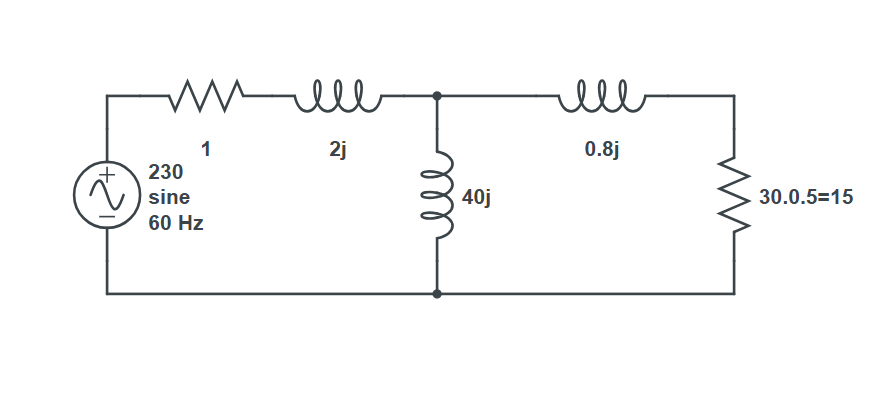
\includegraphics[width=0.9\textwidth]{circuit.png}
   \caption{Circuit for problem 16.15}
   \label{nem_ngang}
   \end{figure}
Synchronous speed (no-load speed):
$$n_{s}=\frac{120.60}{4}=1800$$
The slip:
$$s=\frac{n_{s}-n_{m}}{n_{s}}=\frac{1800-1740}{1800}=\frac{1}{30}$$
$$Z_{s}=1+2j+\frac{(0,8j+15)40j}{0,8j+15+40j}=13,7+7.45j=15.6\angle 28,55\degree$$
Power factor $=\cos{28.55\degree}=87.84\%$ lagging
$$I_{s}=\frac{V_{s}}{Z_{s}}=\frac{230\angle 0\degree}{15,6\angle 28,55\degree}=14,74\angle -28,55\degree$$
Line current:
$$I_{line}=\sqrt{3}I_{s}=14,74\sqrt{3}=25,53 (A rms)$$
\section*{Problem 16.21:}
A $3$ $hp$ six-pole $60$ $Hz$ delta-connected 
three-phase induction motor is rated for 
$1140$ $rpm$, $220$ $V$ $rms$, and $8,58$ $A$ $rms$ (line 
current) at an $80$ percent lagging power 
factor. Find the full-load efficiency.
\\ \textbf{Solution:}
$$P_{out}=2.746=1492$$
We have:
$$V_{s}=V_{line}$$
$$I_{s}=\frac{I_{line}}{\sqrt{3}}$$
\begin{align*}
P_{in}&=3I_{s}V_{s}\cos{\theta}=\frac{3I_{line}}{\sqrt{3}}V_{line}\cos{\theta}=\sqrt{3}I_{line}V_{line}\cos{\theta}\\&=\sqrt{3}.5,72.220.0,8=1743,69 (W)
\end{align*}
The efficiency is:
$$\eta=\frac{1492}{1743,69}.100\%=85,57\%$$
\section*{Problem 16.31:}
A certain four-pole $440$ $V$ $rms$ $60$ $Hz$ three
phase delta-connected induction motor has
 $R_{s} = 0,12\Omega, X_{s} = 0,30\Omega,X_{m} = 7,5\Omega,R_{r}^{'} = 0,10\Omega,
 X_{r}^{'}= 0,20 \Omega$.
 Under load, the machine operates with a 
slip of $4$ percent and has rotational losses of 
$2$ $kW$. Determine the power factor, output 
power, copper losses, output torque, and 
efficiency.
\\ \textbf{Solution:}
$$P_{out}=2.746=1492W$$
Synchronous speed:
$$n_{s}=\frac{120f}{p}=\frac{120.60}{8}=900(rpm)$$
Slip:
$$s=\frac{n_{s}-n_{m}}{n_{s}}=\frac{900-850}{900}=0.0556$$
Frequency of motor currents:
$$f_{r}=s.f_{s}=0.0556.60=3.33 (Hz)$$
Developed power:
$$P_{dev}=3\frac{1-s}{s}.R_{r}^{'}I_{r}^{2}=\frac{1-s}{s}P_{r}$$
Also: $P_{dev}=P_{out}+P_{rot}=1492+100=1592 (W)$
$$\Rightarrow P_{r}=\frac{s}{1-s}P_{dev}=\frac{0.0556}{1-0.0556}.1592=93,726(W)$$
\section*{Problem 16.42:}
A six-pole $60$ $Hz$ synchronous motor is operating with a developed power of $5$ $hp$ and a torque angle of $5 \degree$. 
Find the speed and developed torque. Suppose that the load increases such that the developed torque doubles.
Find the new torque angle. Find the pull-out torque and maximum developed power for this machine.
\\ \textbf{Solution:}
\\ From the problem description we have:
$$P=6W, f=60 Hz, P_{dev1}=5hp, \delta_{1}=5\degree$$
\\The developed power in watts is:
$$P_{dev1}=5.746=3730$$
The synchronous speed is:
$$n_{s}=\frac{120f}{p}=\frac{120.60}{6}=1200 rpm$$
The developed torque is:
$$T_{dev1}=\frac{P_{dev1}}{\omega s}=\frac{P_{dev1}}{ns}.\frac{60}{2\pi}=\frac{3730.1200}{1200}.\frac{60}{2\pi}=29,682 Nm$$
The developed torque is doubled, so we can write:
$$T_{dev2}=2T_{dev1}=2.29,682=59,635 Nm$$
Recall that developed torque is given by following equation:
$$T_{dev}=K.B_{r}.B_{total}.\sin{\delta}$$
We can use the previous equation to determine new torque angle $\delta_{2}$. But first, we have to calculate the value of constants $K.B_{r}.B_{total}$.
For the $T_{dev1}$ and $\delta_{1}$, we have:
$$T_{dev1}=K.B_{r}.B_{total}.\sin{\delta_{1}}\Rightarrow K.B_{r}.B_{total}=\frac{T_{dev1}}{\sin{\delta_{1}}}=\frac{29,682}{\sin{5\degree}}=340,563$$
For the $T_{dev2}$ and $\delta_{2}$, we can write:
$$T_{dev2}=K.B_{r}.B_{total}.\sin{\delta_{2}}\Rightarrow \sin{\delta_{2}}=\frac{59,635}{340,563}=0,175$$
Finally, the torque angle is:
$$\delta_{2}=\arcsin{0,175}=10,08\degree$$
The pull out torque occurs for torque angle $\delta=90\degree$
$$T_{pull-out}=K.B_{r}.B_{total}.\sin{90\degree}=340,563$$
The maximum developed power is defined as follows:
$$P_{max}=T_{pull-out}\omega.s=T_{pull-out}.ns\frac{2\pi}{60}=42976,41 W$$
\end{document}
